\documentclass[10pt,conference]{IEEEtran}
\IEEEoverridecommandlockouts

\usepackage{cite}
\usepackage{amsmath,amssymb,amsfonts}
\usepackage{graphicx}
\usepackage{booktabs}
\usepackage{array}
\usepackage{tikz}
\usetikzlibrary{arrows.meta,positioning,calc,backgrounds}
\usepackage{xcolor}
\usepackage[hidelinks]{hyperref}
\usepackage{url}

\newcommand{\code}[1]{\texttt{\small #1}}

\title{SKED: Sharing a Single Global KV Cache Across All Decoder Layers\\ for Memory-Bound Long-Context Inference}

\author{
\IEEEauthorblockN{SKED Project}
\IEEEauthorblockA{\textit{Design note and preliminary measurements}\\
Code: Apache-2.0 \quad|\quad Paper: CC BY 4.0\\
\texttt{https://github.com/3440340143/sked}}
}

\begin{document}
\maketitle

\begin{abstract}
Long-context inference is bounded by two distinct memory costs: the static weight
footprint of the model and the dynamic key--value (KV) cache, which in a standard
Transformer grows with both sequence length and layer count. We describe \textbf{SKED}
(\emph{Shared-KV Encoder--Decoder}), a design that attacks both costs simultaneously by
combining three existing ingredients: (i) 1.58-bit ternary weights with a corrected
straight-through estimator, (ii) a causal encoder that emits \emph{one} global KV
projection reused by every decoder layer through causally-masked cross-attention, and
(iii) sliding-window local attention in both stacks so that local KV stays
$O(W)$ rather than $O(L)$. We additionally propose four extensions that, to our
knowledge, are not standard in this combination: chunked global KV projection,
low-rank per-layer KV adapters over the shared base, phase-asymmetric expert
activation, and dual-tier sliding windows.

This is a \emph{design note with small-scale verification}, not a validated result.
The architecture is not trained at scale. We report a runnable reference
implementation with mask-correctness tests, an analytical memory accounting that is
checked against the live module tree, and four CPU-scale preliminary experiments. Two
of them establish concrete properties of the mechanism. A multi-query associative-recall
ablation shows that the shared cross-attention path is what carries long-range
information: with it, accuracy is $1.000$; a windowed control identical except that the
path is removed scores $0.388$. The same ablation shows the encoder needs no dense
layer --- a fully windowed encoder matches a fully dense one --- so the prefill path
stays free of an $O(L^2)$ term. Two results are unfavourable and we state them rather
than omit them: on CPU the ternary path is 1.3--2.1$\times$ \emph{slower} than fp32,
because commodity hardware has no native ternary instruction, and the recall task is
solved only at toy scale (6 pairs, $2{+}2$ layers, 1500 steps), which is far from
evidence that the architecture is competitive.
\end{abstract}

\begin{IEEEkeywords}
efficient inference, KV cache, ternary weights, sliding-window attention,
encoder--decoder, long context
\end{IEEEkeywords}

\section{Introduction}

Two walls are hit simultaneously when serving a language model at long context.

\textbf{Static weights.} Mixture-of-Experts (MoE) models keep the entire expert pool
resident in memory even though only a fraction is active per token. A 1.58-bit ternary
representation~\cite{bitnet158} reduces this by roughly $8\times$ relative to BF16
before any sparsity is exploited.

\textbf{Dynamic KV.} A conventional Transformer stores a separate key/value tensor per
layer, so the cache grows as $O(N_{\text{layers}} \cdot L \cdot d)$. At $L = 128$k this
dominates. Two established families of remedies exist: low-rank KV compression, as in
MLA~\cite{deepseekv3}, and cross-layer KV sharing, as in the causal
encoder--decoder (CED) line of work~\cite{yoco}. Sliding-window
attention~\cite{longformer,mistral,gemma2} attacks a different axis, bounding the
\emph{local} cache but leaving a global path to be accounted for.

SKED is an exercise in combining these ideas under one accounting. Its contribution
claim is deliberately narrow: \emph{the specific combination and its parameterisation},
together with a reference implementation in which the parts that are easy to get wrong
--- the straight-through estimator and the cross-attention mask --- are handled
correctly and covered by tests. We do not claim novelty for any individual component.

The rest of the note is organised as follows. Section~\ref{sec:bg} fixes notation and
situates the work. Section~\ref{sec:arch} describes the architecture.
Section~\ref{sec:ext} proposes four extensions. Section~\ref{sec:exp} reports four
preliminary experiments. Section~\ref{sec:limits} lists what is \emph{not} established.
Section~\ref{sec:conc} concludes.

\section{Background and Notation}\label{sec:bg}

Let $L$ be the sequence length, $d$ the model width, $H$ the number of heads,
$d_h = d/H$ the head dimension, $N_e$/$N_d$ the encoder/decoder depth, and $W$ the
sliding-window width.

\paragraph{Ternary weights.} BitNet b1.58~\cite{bitnet158} rounds weights to
$\{-1,0,+1\}$ after scaling by $\gamma = \frac{1}{d}\lVert W \rVert_1$. Storage is
1.58 bits per weight in the limit, 2 bits in practice. Matmuls become additions. The
difficulty is trainability: the quantiser has zero gradient almost everywhere, so a
straight-through estimator (STE) is required.

\paragraph{Cross-layer KV sharing.} In a causal encoder--decoder layout the encoder
runs a full causal pass and the decoder attends to the encoder's final-layer states
through cross-attention. If the projection is performed \emph{once}, every decoder
layer reads the same $K_0, V_0$, and the cache drops from $N_d$ copies to one. This is
the mechanism SKED borrows~\cite{yoco}.

\paragraph{The masking hazard.} The encoder is causal, so $K_0[j]$ depends only on
tokens $\leq j$. If decoder position $i$ is allowed to attend to $j > i$, it reads a
summary of the token it is about to predict; training loss collapses while generative
ability is destroyed. Any implementation of this family must mask the cross-attention
path. This is the single most failure-prone part of the design and is where our
reference implementation concentrates its tests.

\paragraph{What the shared cache does \emph{not} need.} It is tempting to require that
the encoder itself have a global receptive field, so that each $K_0[j]$ summarises the
whole prefix. It does not. The decoder cross-attends over the entire $K_0$ set, and
position $p$ appears in $K_0[p \dots p+W-1]$; since $p \leq i$ whenever $p$ is in the
past, $K_0[p]$ always exists and every position stays addressable. A windowed encoder
therefore suffices, and Section~\ref{sec:exp} confirms this by measurement. The
distinction matters because it is the difference between a prefill path with an
$O(L^2)$ term and one without.

\section{The SKED Architecture}\label{sec:arch}

\begin{figure*}[t]
\centering
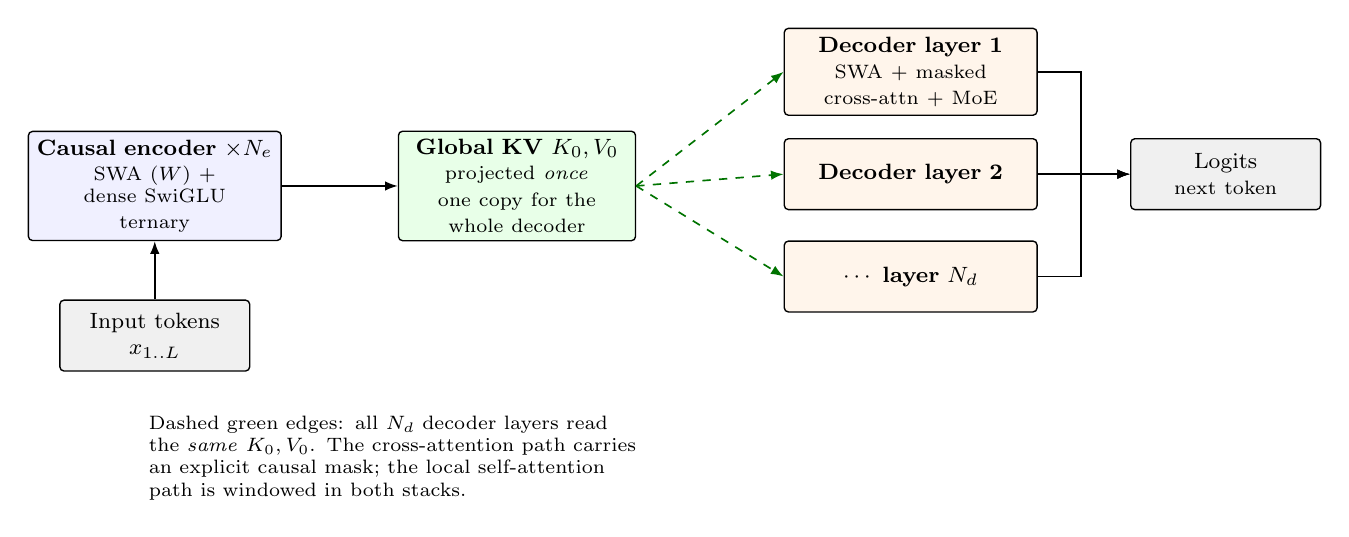
\begin{tikzpicture}[
  font=\footnotesize,
  box/.style={draw, rounded corners=1.5pt, align=center, inner sep=3pt,
              minimum height=9mm, text width=30mm, line width=0.5pt},
  enc/.style={box, fill=blue!6},
  dec/.style={box, fill=orange!8},
  kvb/.style={box, fill=green!9, text width=28mm},
  io/.style={box, fill=black!6, text width=22mm},
  ar/.style={-{Latex[length=1.6mm]}, line width=0.6pt},
  shr/.style={-{Latex[length=1.6mm]}, line width=0.6pt, dashed, color=green!45!black}
]
\node[io]  (tok) at (0,0)      {Input tokens\\$x_{1..L}$};
\node[enc] (enc) at (0,1.9)    {\textbf{Causal encoder} $\times N_e$\\[1pt]
                                \scriptsize SWA ($W$) + dense SwiGLU\\\scriptsize ternary};
\node[kvb] (gkv) at (4.6,1.9)  {\textbf{Global KV} $K_0,V_0$\\[1pt]
                                \scriptsize projected \emph{once}\\\scriptsize one copy for the whole decoder};
\node[dec] (d1) at (9.6,3.35)  {\textbf{Decoder layer 1}\\\scriptsize SWA + masked cross-attn + MoE};
\node[dec] (d2) at (9.6,2.05)  {\textbf{Decoder layer 2}};
\node[dec] (d3) at (9.6,0.75)  {$\cdots$ \textbf{layer $N_d$}};
\node[io]  (out) at (13.6,2.05) {Logits\\\scriptsize next token};

\draw[ar] (tok) -- (enc);
\draw[ar] (enc) -- (gkv);
\draw[shr] (gkv.east) -- (d1.west);
\draw[shr] (gkv.east) -- (d2.west);
\draw[shr] (gkv.east) -- (d3.west);
\draw[ar] (d1.east) -- ++(0.55,0) |- (out.west);
\draw[ar] (d2.east) -- (out.west);
\draw[ar] (d3.east) -- ++(0.55,0) |- (out.west);

\node[align=left, font=\scriptsize, text width=62mm, anchor=north west]
     at (-0.2,-0.9) {Dashed green edges: all $N_d$ decoder layers read the
     \emph{same} $K_0,V_0$. The cross-attention path carries an explicit causal
     mask; the local self-attention path is windowed in both stacks.};
\end{tikzpicture}
\caption{SKED dataflow. The encoder produces a single global KV projection; every
decoder layer reuses it under a causal mask. Local self-attention in both stacks is
sliding-window, so only the shared global cache grows with $L$.}
\label{fig:arch}
\end{figure*}

Figure~\ref{fig:arch} shows the layout.

\subsection{Ternary backbone}

Every projection (attention $Q/K/V/O$, dense SwiGLU, MoE experts, global KV
projection) is a \code{BitLinear158} layer. We use the following estimator:
\begin{equation}
w_{\text{ste}} \;=\; \underbrace{\hat{w}_q}_{\text{detach}} \;+\;
\mathbb{1}\!\left[\,|w_s| \le 1.5 \,\right] \cdot \left( w_s - w_s^{\text{detach}} \right),
\label{eq:ste}
\end{equation}
where $w_s = w/\gamma$ and $\hat{w}_q = \mathrm{clip}(\mathrm{round}(w_s),-1,1)$.
The forward value is then \emph{exactly} $\hat{w}_q$ --- a genuine ternary
value --- while the backward pass sees the indicator-masked identity.

This is worth stating explicitly because the common shorthand
$w + (\hat{w}_q - w)^{\text{detach}}$ leaves a residual floating-point term in the
forward pass. The forward computation is then not ternary at all, and the whole point
of the quantisation is silently lost. Equation~\ref{eq:ste} is covered by a test that
asserts the forward output is exactly ternary (Section~\ref{sec:exp}).

\subsection{Shared global KV}

The encoder output $H \in \mathbb{R}^{L \times d}$ is projected once:
\begin{equation}
K_0 = W^K_g H, \qquad V_0 = W^V_g H,
\end{equation}
with $W^K_g, W^V_g$ ternary. Every decoder layer $l$ computes
\begin{equation}
\text{CrossAttn}_l(Q_l, K_0, V_0), \qquad
Q_l = W^Q_l \, \mathrm{RMSNorm}(x_l),
\end{equation}
so there is one $K_0,V_0$ for the whole decoder rather than $N_d$ independent caches.

\subsection{Causal cross-attention}

The mask is written in \emph{absolute index} form:
\begin{equation}
q_{\text{idx}} = \mathrm{arange}(L_k - L_q,\, L_k), \qquad
M_{ij} = \mathbb{1}[\, k_{\text{idx},j} \le q_{\text{idx},i} \,].
\label{eq:mask}
\end{equation}
Because the query indices are derived from the \emph{cache} length rather than from a
per-call local offset, the same expression is correct in both regimes: full prefill
($L_q = L$) and incremental decoding ($L_q = 1$, $L_k$ growing). Writing the mask as a
local lower triangle instead is a common bug: it is correct during prefill and silently
wrong during decode, when every query is at the last position and a local mask
degenerates to ``attend to everything''.

We also apply soft-capping to the cross-attention scores,
$s \mapsto c\tanh(s/c)$ with $c = 50$, following~\cite{gemma2}, and a logit soft-cap
$c=30$ at the output head.

\subsection{Sliding-window local attention}

Both stacks use causal sliding-window attention with width $W$. The stored cache is
explicitly truncated,
\begin{equation}
\text{cache} \leftarrow \text{cache}[:,\,-W\!:\!,:],
\end{equation}
so local KV is $O(W)$ and constant in $L$. This is asserted by a test that checks the
cache length after a long forward pass.

Applying the window to the encoder as well as the decoder is a deliberate choice and
not an obvious one. Section~\ref{sec:exp} measures what it costs: nothing. The
alternative --- one dense causal layer at the encoder tail --- buys no accuracy on the
recall task and reintroduces an $O(L^2)$ prefill term, so the windowed encoder is the
configuration we recommend.

\subsection{Parameterisation}

The spec configuration is $d=2048$, $H=16$, $d_h=128$, $N_e=N_d=16$, encoder FFN
$5632$, decoder experts $32$ with top-$k=4$ and expert hidden $2816$, $W=512$, and a
weight-tied $128$k vocabulary. This yields:

\begin{table}[t]
\centering
\caption{Static weight accounting, spec configuration. Checked against the live module
tree on a meta device; ternary weights are counted at 2 bits, everything else at its
own dtype width. Arithmetic, not measurement.}
\label{tab:params}
\small
\begin{tabular}{@{}lrr@{}}
\toprule
Component & Parameters & Footprint \\
\midrule
Ternary backbone (BitLinear) & 10.09\,B & 2.350\,GiB \\
Embedding/head (tied), fp32 & 0.263\,B & 0.984\,GiB \\
Norms, scales, biases & --- & $\sim$0.01\,GiB \\
\midrule
\textbf{Total} & \textbf{10.356\,B} & \textbf{3.333\,GiB} \\
\bottomrule
\end{tabular}
\end{table}

Table~\ref{tab:params} makes one point that is easy to get wrong: the tied
embedding/output head is only $2.6\%$ of the parameters but $30\%$ of the footprint.
Storing it in BF16 rather than fp32 recovers $0.49$\,GiB, bringing the total to
$\approx 2.85$\,GiB. Any claim of ``under 3\,GB'' therefore depends on the embedding
dtype, and we state the dtype rather than the headline.

\section{Proposed Extensions}\label{sec:ext}

The following four mechanisms are proposals. None has been implemented or validated in
the prototype; we describe them because they are the directions we believe are worth
testing, and we flag the risk attached to each.

\subsection{Chunked global KV (CGKV)}

\emph{Problem.} The reference implementation materialises an explicit $[L_q \times L_k]$
mask. At $L=128$k the mask alone is $O(L^2)$; the implementation is only usable for
short sequences.

\emph{Proposal.} Run the encoder over fixed-size chunks of $C$ tokens. Chunk $c$ emits
its own global KV segment $K_0^{(c)}, V_0^{(c)}$, appended to an append-only cache.
Decoder cross-attention for a token in chunk $c$ attends to segments $1..c$ with a
banded mask. Peak mask memory becomes $O(C \cdot W)$ rather than $O(L^2)$, and the
cache becomes streamable: a chunk can be encoded and evicted without re-running the
encoder.

\emph{Risk.} The encoder's representation of position $i$ now depends on which chunk
boundary it falls near, which introduces a periodic artefact. Whether this hurts
quality is an empirical question.

\subsection{Low-rank per-layer KV adapters over the shared base}

\emph{Problem.} Pure sharing forces all $N_d$ decoder layers to read an identical
$K_0, V_0$. Different layers plausibly want different views of the context; giving each
layer its own cache is exactly what we are trying to avoid.

\emph{Proposal.} Keep one shared base and add a low-rank residual per layer:
\begin{equation}
K_l = K_0 + A^K_l B^K_l K_0, \qquad V_l = V_0 + A^V_l B^V_l V_0,
\end{equation}
with $A_l \in \mathbb{R}^{d \times r}$, $B_l \in \mathbb{R}^{r \times d}$, $r \ll d$.
The adapters are applied to the \emph{projected} KV, so they cost
$4 N_d d r$ parameters in total --- negligible at $r = 64$ --- and no extra cache.
This is a deliberate middle point between ``one shared cache'' (cheap, low capacity)
and ``one cache per layer'' (expensive, high capacity).

\emph{Risk.} If the adapters absorb too much, the shared base degrades into a
convenient initialisation and the memory argument still holds but the mechanism is no
longer doing the work; an ablation with $r$ swept over $\{0, 16, 64, 256\}$ would
separate the two.

\subsection{Phase-asymmetric expert activation (PAEA)}

\emph{Observation.} Prefill is compute-bound; decode is memory-bandwidth-bound. The two
phases want different compute/memory trade-offs, yet most MoE designs use one static
expert configuration for both.

\emph{Proposal.} Make the FFN asymmetric by phase and by depth: a dense SwiGLU in the
encoder (which only ever runs during prefill), MoE in the decoder, and within the
decoder a depth-dependent active-expert count --- fewer experts in early layers, more
in later layers. The rationale is that early layers do representational work that is
shared across tokens, while later layers carry the knowledge that benefits from
specialisation, and decode-time FLOPs are cheap relative to the memory traffic.

\emph{Risk.} This is the weakest of the four proposals. It rests on an assumption about
layer-wise specialisation that we have not tested, and the router's load-balancing
behaviour under a depth-varying $k$ is non-obvious.

\subsection{Dual-tier sliding window (DTSW)}

\emph{Proposal.} Alternate the window width across decoder layers, $W_s$ on even layers
and $W_l$ on odd layers ($W_s \ll W_l$). The local cache then costs one $W_l$ buffer
plus one $W_s$ buffer, but the effective receptive field is hierarchical: a token two
layers down can reach $W_s + W_l$ positions back. This is cheaper than a uniform $W_l$
and more expressive than a uniform $W_s$.

\emph{Risk.} The gain over a uniform window of the average width is likely small, and
Gemma~2~\cite{gemma2} already interleaves local and global layers; the distinction is
that we interleave two \emph{local} tiers to keep the global path the sole unbounded
one.

\section{Preliminary Experiments}\label{sec:exp}

\emph{Scope statement.} All experiments below are small-scale CPU runs on a research
prototype. They probe \emph{internal consistency, scaling behaviour, and one mechanism
ablation}. They say nothing about model quality: no language-modelling benchmark is
reported and no model of useful size has been trained. Code and raw JSON are in the
repository.

\subsection{Setup and correctness}

The prototype used for the memory and matmul measurements is $d=128$, $H=4$,
$N_e=N_d=2$, encoder FFN $256$, MoE hidden $192$ with $8$ experts and top-$2$,
$W=256$. The recall ablation of Section~\ref{sec:exp} uses a smaller
$d=64$ configuration with fp32 weights, for the reason given there. Ten smoke tests
pass, covering: forward output is exactly ternary; gradients flow; no NaN/Inf;
\emph{no future leak} in either stack; causality holds beyond the window; incremental
decode is numerically equal to a full forward pass; the decode path respects window
truncation; the MoE balancing bias updates; and the parameter accounting of
Table~\ref{tab:params} reproduces.

The last two tests matter more than they look. ``Incremental decode equals full
forward'' is the property that the absolute-index mask of Eq.~\ref{eq:mask} exists to
protect; a local-triangle mask passes prefill and fails this test.

\subsection{KV footprint versus sequence length}

\begin{figure}[t]
\centering
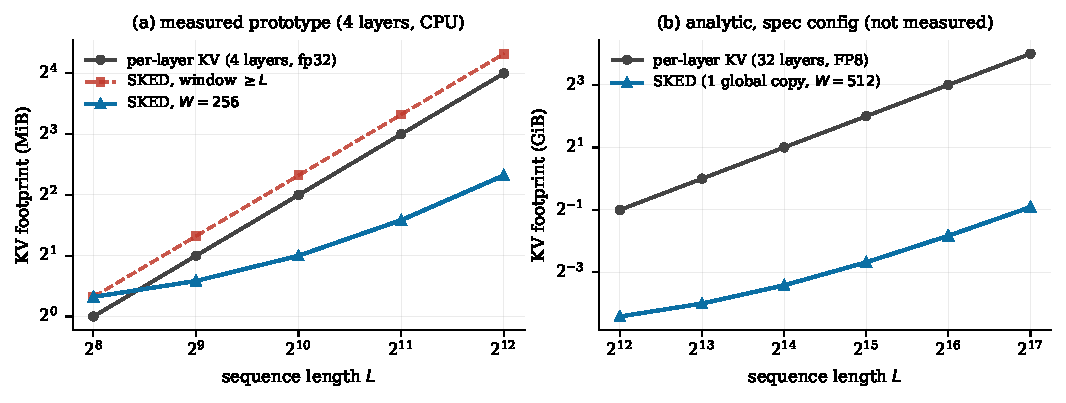
\includegraphics[width=\columnwidth]{figures/fig_kv_scaling.pdf}
\caption{(a) Measured KV footprint of the prototype. The per-layer baseline is
$N_{\text{layers}}$ separate caches; SKED replaces them with one shared global cache
plus constant-size windowed local caches. (b) Analytic extrapolation to the spec
configuration. Panel (b) is arithmetic, not measurement.}
\label{fig:kv}
\end{figure}

Figure~\ref{fig:kv}(a) reports the live cache tensor sizes. Three regimes are compared:
a per-layer baseline ($N_e + N_d = 4$ separate fp32 caches), SKED with the window
disabled ($W \ge L$, i.e.\ full causal attention), and SKED with $W = 256$.

At $L = 4096$ the per-layer baseline is $16.0$\,MiB and windowed SKED is
$5.0$\,MiB --- $31\%$. More informative than the ratio is the shape: the local
component of SKED is $1.0$\,MiB at $L = 512$ and still $1.0$\,MiB at $L = 4096$,
confirming that window truncation holds, while the global component grows as $L$ with
slope $1$ rather than slope $N_d$.

The asymptotic claim is arithmetic. With the spec configuration at $L = 128$k in FP8,
the per-layer baseline is $16$\,GiB; SKED is one global cache ($512$\,MiB) plus decoder
local caches ($32$\,MiB), i.e.\ $544$\,MiB, or $3.3\%$. The saving factor is
essentially $N_d$: the global cache is paid for once instead of $N_d$ times. This is
what Fig.~\ref{fig:kv}(b) plots. \textbf{It is a memory-accounting statement, not a
measured speedup}, and it is only meaningful if the shared cache turns out to be
sufficient. Section~\ref{sec:exp} gives a first positive answer to that question at
toy scale; it does not settle it at any scale where the memory saving matters.

\subsection{Ternary matmul cost on commodity hardware}

\begin{figure}[t]
\centering
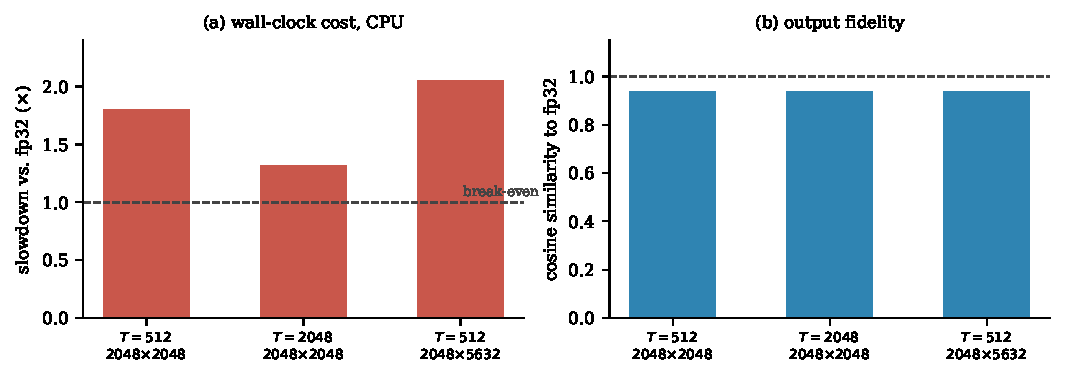
\includegraphics[width=\columnwidth]{figures/fig_ternary.pdf}
\caption{Measured cost and fidelity of the ternary path against fp32, CPU, 16 threads,
random (untrained) weights. (a) The ternary path is \emph{slower} in all three shapes.
(b) Output cosine similarity to the fp32 reference.}
\label{fig:tern}
\end{figure}

This experiment exists to test a claim we would otherwise be tempted to make. Ternary
weights are often described as a throughput win. On commodity hardware they are not.
Figure~\ref{fig:tern}(a): the ternary path is $1.81\times$, $1.32\times$ and
$2.06\times$ \emph{slower} than fp32 for
$(T,d_{\text{in}},d_{\text{out}}) \in \{(512,2048,2048), (2048,2048,2048),
(512,2048,5632)\}$. The reason is structural: mainstream tensor cores expose
FP16/BF16/FP8/INT8/INT4 but no ternary format, so the kernel must dequantise online and
then run a standard GEMM --- paying the quantisation cost without collecting any of the
saving.

Output fidelity is $\cos \approx 0.9376$ in all three shapes. The relative $L_2$ error
is large ($\approx 0.40$); we note that this is measured on \emph{random} weights,
where $\gamma$ is arbitrary and no learned structure exists to absorb the
quantisation, so the absolute error is not indicative of a trained ternary model. We
report the cosine figure and not the relative error as the headline, and we flag that
even the cosine figure is only meaningful as a sanity check that the estimator is not
degenerate.

The practical conclusion is narrow but firm: \textbf{the ternary advantage of SKED is a
\emph{storage} advantage, not a compute advantage}, on any hardware without a
purpose-built ternary kernel (e.g.\ bitnet.cpp on AVX-512, or T-MAC-style lookup
tables).

\subsection{Does the shared global KV path carry long-range information?}

\begin{figure}[t]
\centering
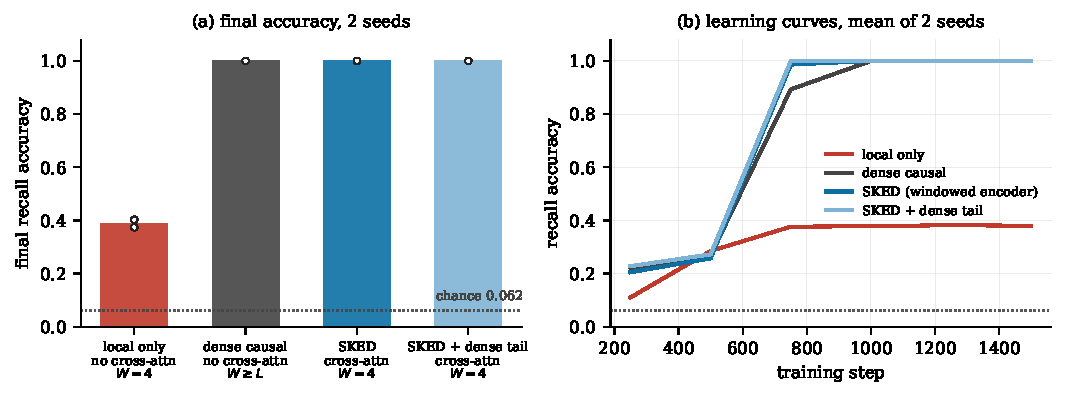
\includegraphics[width=\columnwidth]{figures/fig_ablation.pdf}
\caption{Multi-query associative recall, 6 key/value pairs, $W=4$, fp32 weights,
$2{+}2$ layers, 1500 steps, two seeds. The queried pair sits outside the local window,
so a correct answer requires the shared KV path. (a) Final accuracy; dots are
individual seeds. (b) Learning curves. Removing cross-attention while keeping the same
window (\code{local\_only}) costs $0.61$ accuracy; the encoder's receptive field costs
nothing.}
\label{fig:ablation}
\end{figure}

The memory accounting above is arithmetic; whether the mechanism \emph{works} is not.
We use multi-query associative recall~\cite{recall}: a sequence of $N$ unique
key/value pairs interleaved as $[k_0,v_0,k_1,v_1,\dots]$, a separator, then a query
key; only the final position is scored. The queried pair is up to $2N-1$ tokens back,
far outside $W=4$, so the answer can only arrive through the shared KV path.

Four variants are compared at matched parameter count. Two control for the presence of
the path: \code{local\_only} (window $W{=}4$, no cross-attention) and \code{dense\_causal}
(window $\geq L$, no cross-attention, i.e.\ an ordinary full-attention model). Two vary
the encoder's receptive field while keeping cross-attention: \code{sked\_tail0}
(fully windowed encoder) and \code{sked\_tail1} (one dense causal layer at the encoder
tail).

\emph{Quantisation is held out of this experiment.} All four variants use fp32 weights.
An earlier version of this ablation ran with ternary weights at $d=64$ and
\emph{none} of the variants learned the task --- including the full-attention upper
bound, which scored $0.271$. That is a statement about the quantiser at toy scale, not
about the architecture, and mixing the two axes makes the ablation uninterpretable. We
therefore gate on the upper bound: if \code{dense\_causal} does not solve the task,
nothing downstream is worth measuring. It does, reaching $1.000$ by step 1000.

Results (Table~\ref{tab:ablation}, Fig.~\ref{fig:ablation}):

\begin{table}[t]
\centering
\caption{Recall ablation. Mean over two seeds; individual seeds in parentheses.
All variants are fp32 with matched parameter count.}
\label{tab:ablation}
\small
\begin{tabular}{@{}llc@{}}
\toprule
Variant & Encoder & Accuracy \\
\midrule
\code{dense\_causal} & dense & $1.000$ \,(1.000, 1.000) \\
\code{local\_only}   & windowed & $0.388$ \,(0.403, 0.374) \\
\code{sked\_tail0}   & windowed & $1.000$ \,(1.000, 1.000) \\
\code{sked\_tail1}   & dense tail & $1.000$ \,(1.000, 1.000) \\
\bottomrule
\end{tabular}
\end{table}

\begin{enumerate}
\item \textbf{The shared path is doing the work.} \code{sked\_tail0} reaches $1.000$
with a local window of 4 tokens, while \code{local\_only} --- identical except that the
cross-attention path is removed --- stalls at $0.388$. The gap is the mechanism.
\item \textbf{The encoder's receptive field is irrelevant.} \code{sked\_tail0} (fully
windowed), \code{sked\_tail1} (dense tail) and \code{dense\_causal} (fully dense) all
score $1.000$. Adding a dense layer to the encoder buys nothing, so the encoder can
stay fully windowed and the prefill path retains no $O(L^2)$ term.
\end{enumerate}

The second point is worth dwelling on, because the opposite conclusion is easy to
reach. A training-free probe that perturbs token 0 and measures the induced change in
the last entry of the shared cache returns \emph{exactly} $0.000000$ for a windowed
encoder, against $0.069$ with a dense tail
(\code{results/exp6\_receptive\_field.json}). That is a real effect and it invites the
inference that a windowed encoder cannot serve as a global cache. The inference is
wrong, and the ablation is what shows it: the decoder reads the \emph{entire} $K_0$
set, and position $p$ lives in $K_0[p \dots p+W-1]$, so no position becomes
unreachable merely because one particular cache entry cannot see the sequence start.
We report the probe alongside the ablation because the probe alone would have led us
to the wrong design.

\paragraph{What this does and does not show.} It shows that the cross-attention path
transmits long-range information and that the encoder need not be dense. It does
\emph{not} show that SKED is competitive: the task is synthetic, the model is
$2{+}2$ layers at $d=64$, and $1.000$ on 6 pairs says nothing about language
modelling. Both \code{sked} variants tie the dense upper bound here; whether they
match it on real data, where the shared cache is a genuine bottleneck, is the open
question.

\section{Threats to Validity and Limitations}\label{sec:limits}

We list these at length because the design is otherwise easy to oversell.

\begin{enumerate}
\item \textbf{No training at scale.} The only trained artifact is the $2{+}2$ layer
recall probe of Section~\ref{sec:exp}. Every quality claim about the spec configuration
remains a design target.
\item \textbf{No language-modelling evaluation.} No perplexity, no benchmark. The
recall task is a mechanism probe, not a capability measure.
\item \textbf{The prefill cost of the cross-attention mask is unsolved in the reference
code.} The encoder can be kept free of an $O(L^2)$ term (Section~\ref{sec:exp}), but
the decoder's causal cross-attention over the full $K_0$ set still materialises an
$O(L^2)$ mask, so the implementation cannot run at the lengths where the KV argument
matters. CGKV and a fused sliding-window kernel are proposals, not implementations.
\item \textbf{No RoPE extrapolation.} $\theta = 10^4$ will not reach $128$k; YaRN/NTK
scaling or long-context annealing is required and is absent.
\item \textbf{Optimiser compatibility unverified.} The interaction of Muon's
Newton--Schulz orthogonalisation with the indicator-masked STE of Eq.~\ref{eq:ste} is
untested; weights near the $\pm 1.5$ threshold may chatter. AdamW is the safe default
until ablated.
\item \textbf{No ternary compute win on commodity hardware}, measured and reported
above. The storage saving is real; the speedup is not, absent a custom kernel.
\item \textbf{The ablation is not at a scale where it decides anything.} At $6$ pairs,
$2{+}2$ layers and $1500$ steps, \code{sked} ties a fully dense model. That the shared
cache is \emph{sufficient} is a much stronger claim than that it is \emph{not
immediately harmful}, and only the former would justify the memory argument. It is not
known whether the combination beats (i) each component used alone at scale, or (ii) a
dense model with the same active parameter count on real data. Until that exists, SKED
should be read as a hypothesis.
\item \textbf{Training cost.} A $10.36$\,B model at multi-trillion-token scale needs a
large cluster. ``Consumer-GPU friendly'' applies to \emph{inference} only.
\item \textbf{Knowledge-intensive tasks may suffer.} Aggressive ternary discretisation
plausibly harms long-tail factual recall. The design expects rule-governed tasks
(mathematics, code) to degrade less, but this is an expectation, not a finding.
\end{enumerate}

\section{Conclusion and Outlook}\label{sec:conc}

SKED combines ternary weights, a single shared global KV cache, and sliding-window
local attention under one accounting. Its reference implementation is mask-correct and
test-covered; its memory argument is arithmetic and reproduces against the live module
tree; its compute argument is \emph{false} on commodity hardware and we say so; and its
central mechanism --- whether one shared global KV carries long-range information --- is
supported by the toy ablation of Section~\ref{sec:exp}, which is a first check rather
than a demonstration at scale. That same ablation removes a cost we had expected to
pay: the encoder needs no dense layer, so the prefill path carries no $O(L^2)$ term
from the encoder.

Two optimisation levers seem most promising beyond the four proposals above. First,
\emph{speculative decoding composes unusually well with this layout}: a draft model can
reuse the same encoder pass and the same global KV, so the drafting cost is close to
the marginal cost of a decoder step. Second, quantising the global cache itself to the
same low-bit family as the backbone would remove the FP16 dequantisation step from the
attention path --- but, as Section~\ref{sec:exp} shows, that only pays off with a
kernel that can consume the low-bit format directly.

The next concrete step is not more architecture. It is the ablation of
Section~\ref{sec:limits}, item 7, at a scale where it is decidable.

\begin{thebibliography}{9}

\bibitem{bitnet158}
S.~Ma, H.~Wang, L.~Ma, L.~Wang, W.~Wang, S.~Huang, L.~Dong, R.~Wang, J.~Xue, and
F.~Wei, ``The era of 1-bit LLMs: All large language models are in 1.58 bits,''
\emph{arXiv:2402.17764}, 2024.

\bibitem{deepseekv3}
DeepSeek-AI, ``DeepSeek-V3 technical report,'' \emph{arXiv:2412.19437}, 2024.

\bibitem{deepseekr1}
DeepSeek-AI, ``DeepSeek-R1: Incentivizing reasoning capability in LLMs via
reinforcement learning,'' \emph{arXiv:2501.12948}, 2025.

\bibitem{yoco}
Y.~Sun, A.~Dong, S.~Huang, S.~Ma, Q.~Xia, J.~Xue, Y.~Wang, and F.~Wei,
``You only cache once: Decoder--decoder architectures for language models,''
\emph{arXiv:2405.05254}, 2024.

\bibitem{gemma2}
Gemma Team, ``Gemma 2: Improving open language models at a practical size,''
\emph{arXiv:2408.00118}, 2024.

\bibitem{mistral}
A.~Q. Jiang \emph{et al.}, ``Mistral 7B,'' \emph{arXiv:2310.06825}, 2023.

\bibitem{longformer}
I.~Beltagy, M.~E. Peters, and A.~Cohan, ``Longformer: The long-document
transformer,'' \emph{arXiv:2004.05150}, 2020.

\bibitem{flashattn2}
T.~Dao, ``FlashAttention-2: Faster attention with better parallelism and work
partitioning,'' \emph{arXiv:2307.08691}, 2023.

\bibitem{recall}
N.~Arora, E.~Eyuboglu, M.~Zhang, A.~Timalsina, S.~Alberti, D.~Zinsley, J.~Zou,
A.~Rudnicky, and C.~R\'e, ``Simple linear attention language models balance the
recall--throughput tradeoff,'' \emph{arXiv:2402.18668}, 2024.

\end{thebibliography}

\end{document}